\documentclass[twoside]{book}

% Packages required by doxygen
\usepackage{fixltx2e}
\usepackage{calc}
\usepackage{doxygen}
\usepackage[export]{adjustbox} % also loads graphicx
\usepackage{graphicx}
\usepackage[utf8]{inputenc}
\usepackage{makeidx}
\usepackage{multicol}
\usepackage{multirow}
\PassOptionsToPackage{warn}{textcomp}
\usepackage{textcomp}
\usepackage[nointegrals]{wasysym}
\usepackage[table]{xcolor}

% Font selection
\usepackage[T1]{fontenc}
\usepackage[scaled=.90]{helvet}
\usepackage{courier}
\usepackage{amssymb}
\usepackage{sectsty}
\renewcommand{\familydefault}{\sfdefault}
\allsectionsfont{%
  \fontseries{bc}\selectfont%
  \color{darkgray}%
}
\renewcommand{\DoxyLabelFont}{%
  \fontseries{bc}\selectfont%
  \color{darkgray}%
}
\newcommand{\+}{\discretionary{\mbox{\scriptsize$\hookleftarrow$}}{}{}}

% Page & text layout
\usepackage{geometry}
\geometry{%
  a4paper,%
  top=2.5cm,%
  bottom=2.5cm,%
  left=2.5cm,%
  right=2.5cm%
}
\tolerance=750
\hfuzz=15pt
\hbadness=750
\setlength{\emergencystretch}{15pt}
\setlength{\parindent}{0cm}
\setlength{\parskip}{3ex plus 2ex minus 2ex}
\makeatletter
\renewcommand{\paragraph}{%
  \@startsection{paragraph}{4}{0ex}{-1.0ex}{1.0ex}{%
    \normalfont\normalsize\bfseries\SS@parafont%
  }%
}
\renewcommand{\subparagraph}{%
  \@startsection{subparagraph}{5}{0ex}{-1.0ex}{1.0ex}{%
    \normalfont\normalsize\bfseries\SS@subparafont%
  }%
}
\makeatother

% Headers & footers
\usepackage{fancyhdr}
\pagestyle{fancyplain}
\fancyhead[LE]{\fancyplain{}{\bfseries\thepage}}
\fancyhead[CE]{\fancyplain{}{}}
\fancyhead[RE]{\fancyplain{}{\bfseries\leftmark}}
\fancyhead[LO]{\fancyplain{}{\bfseries\rightmark}}
\fancyhead[CO]{\fancyplain{}{}}
\fancyhead[RO]{\fancyplain{}{\bfseries\thepage}}
\fancyfoot[LE]{\fancyplain{}{}}
\fancyfoot[CE]{\fancyplain{}{}}
\fancyfoot[RE]{\fancyplain{}{\bfseries\scriptsize Generated by Doxygen }}
\fancyfoot[LO]{\fancyplain{}{\bfseries\scriptsize Generated by Doxygen }}
\fancyfoot[CO]{\fancyplain{}{}}
\fancyfoot[RO]{\fancyplain{}{}}
\renewcommand{\footrulewidth}{0.4pt}
\renewcommand{\chaptermark}[1]{%
  \markboth{#1}{}%
}
\renewcommand{\sectionmark}[1]{%
  \markright{\thesection\ #1}%
}

% Indices & bibliography
\usepackage{natbib}
\usepackage[titles]{tocloft}
\setcounter{tocdepth}{3}
\setcounter{secnumdepth}{5}
\makeindex

% Hyperlinks (required, but should be loaded last)
\usepackage{ifpdf}
\ifpdf
  \usepackage[pdftex,pagebackref=true]{hyperref}
\else
  \usepackage[ps2pdf,pagebackref=true]{hyperref}
\fi
\hypersetup{%
  colorlinks=true,%
  linkcolor=blue,%
  citecolor=blue,%
  unicode%
}

% Custom commands
\newcommand{\clearemptydoublepage}{%
  \newpage{\pagestyle{empty}\cleardoublepage}%
}

\usepackage{caption}
\captionsetup{labelsep=space,justification=centering,font={bf},singlelinecheck=off,skip=4pt,position=top}

%===== C O N T E N T S =====

\begin{document}

% Titlepage & ToC
\hypersetup{pageanchor=false,
             bookmarksnumbered=true,
             pdfencoding=unicode
            }
\pagenumbering{alph}
\begin{titlepage}
\vspace*{7cm}
\begin{center}%
{\Large My Project }\\
\vspace*{1cm}
{\large Generated by Doxygen 1.8.13}\\
\end{center}
\end{titlepage}
\clearemptydoublepage
\pagenumbering{roman}
\tableofcontents
\clearemptydoublepage
\pagenumbering{arabic}
\hypersetup{pageanchor=true}

%--- Begin generated contents ---
\chapter{Hierarchical Index}
\section{Class Hierarchy}
This inheritance list is sorted roughly, but not completely, alphabetically\+:\begin{DoxyCompactList}
\item \contentsline{section}{alignemnt\+\_\+information}{\pageref{structalignemnt__information}}{}
\item \contentsline{section}{Non\+Primitve\+Type$<$ T $>$}{\pageref{structNonPrimitveType}}{}
\item \contentsline{section}{Primitive\+Type$<$ T $>$}{\pageref{structPrimitiveType}}{}
\item runtime\+\_\+error\begin{DoxyCompactList}
\item \contentsline{section}{Sail\+C\+Error}{\pageref{classSailCError}}{}
\begin{DoxyCompactList}
\item \contentsline{section}{Dimension\+Error}{\pageref{classDimensionError}}{}
\item \contentsline{section}{Dtype\+Error}{\pageref{classDtypeError}}{}
\end{DoxyCompactList}
\end{DoxyCompactList}
\item \contentsline{section}{sail\+:\+:Tensor}{\pageref{classsail_1_1Tensor}}{}
\item \contentsline{section}{Tensor\+Storage}{\pageref{classTensorStorage}}{}
\end{DoxyCompactList}

\chapter{Class Index}
\section{Class List}
Here are the classes, structs, unions and interfaces with brief descriptions\+:\begin{DoxyCompactList}
\item\contentsline{section}{\hyperlink{structalignemnt__information}{alignemnt\+\_\+information} }{\pageref{structalignemnt__information}}{}
\item\contentsline{section}{\hyperlink{classDimensionError}{Dimension\+Error} }{\pageref{classDimensionError}}{}
\item\contentsline{section}{\hyperlink{classDtypeError}{Dtype\+Error} }{\pageref{classDtypeError}}{}
\item\contentsline{section}{\hyperlink{structNonPrimitveType}{Non\+Primitve\+Type$<$ T $>$} }{\pageref{structNonPrimitveType}}{}
\item\contentsline{section}{\hyperlink{structPrimitiveType}{Primitive\+Type$<$ T $>$} }{\pageref{structPrimitiveType}}{}
\item\contentsline{section}{\hyperlink{classSailCError}{Sail\+C\+Error} }{\pageref{classSailCError}}{}
\item\contentsline{section}{\hyperlink{classsail_1_1Tensor}{sail\+::\+Tensor} }{\pageref{classsail_1_1Tensor}}{}
\item\contentsline{section}{\hyperlink{classTensorStorage}{Tensor\+Storage} }{\pageref{classTensorStorage}}{}
\end{DoxyCompactList}

\chapter{Class Documentation}
\hypertarget{structalignemnt__information}{}\section{alignemnt\+\_\+information Struct Reference}
\label{structalignemnt__information}\index{alignemnt\+\_\+information@{alignemnt\+\_\+information}}
\subsection*{Public Attributes}
\begin{DoxyCompactItemize}
\item 
\mbox{\Hypertarget{structalignemnt__information_a092a26827beccdb8eac56dcad0d237aa}\label{structalignemnt__information_a092a26827beccdb8eac56dcad0d237aa}} 
int {\bfseries alignment}
\item 
\mbox{\Hypertarget{structalignemnt__information_a8459d0c5eb17e59e7bac67d5a837cc60}\label{structalignemnt__information_a8459d0c5eb17e59e7bac67d5a837cc60}} 
int {\bfseries dtype\+\_\+size}
\item 
\mbox{\Hypertarget{structalignemnt__information_a973d38a04bc603a21bed6141784014f1}\label{structalignemnt__information_a973d38a04bc603a21bed6141784014f1}} 
int {\bfseries jump}
\end{DoxyCompactItemize}


The documentation for this struct was generated from the following file\+:\begin{DoxyCompactItemize}
\item 
/home/tuckersiegel/\+N\+V\+M\+E/sail/sail/csrc/src/dtypes.\+h\end{DoxyCompactItemize}

\hypertarget{classDimensionError}{}\section{Dimension\+Error Class Reference}
\label{classDimensionError}\index{Dimension\+Error@{Dimension\+Error}}


Inheritance diagram for Dimension\+Error\+:\nopagebreak
\begin{figure}[H]
\begin{center}
\leavevmode
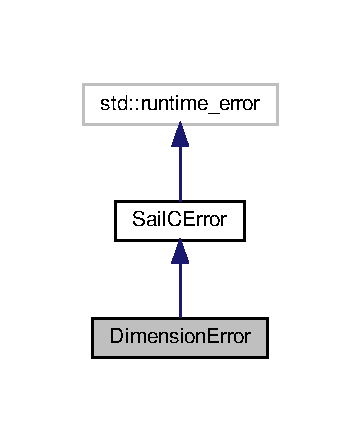
\includegraphics[width=173pt]{classDimensionError__inherit__graph}
\end{center}
\end{figure}


Collaboration diagram for Dimension\+Error\+:\nopagebreak
\begin{figure}[H]
\begin{center}
\leavevmode
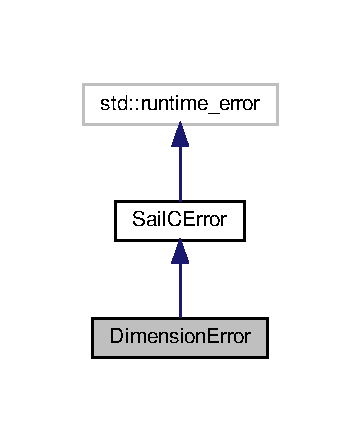
\includegraphics[width=173pt]{classDimensionError__coll__graph}
\end{center}
\end{figure}
\subsection*{Additional Inherited Members}


The documentation for this class was generated from the following file\+:\begin{DoxyCompactItemize}
\item 
/home/tuckersiegel/\+N\+V\+M\+E/sail/sail/csrc/src/error.\+h\end{DoxyCompactItemize}

\hypertarget{classDtypeError}{}\section{Dtype\+Error Class Reference}
\label{classDtypeError}\index{Dtype\+Error@{Dtype\+Error}}


Inheritance diagram for Dtype\+Error\+:\nopagebreak
\begin{figure}[H]
\begin{center}
\leavevmode
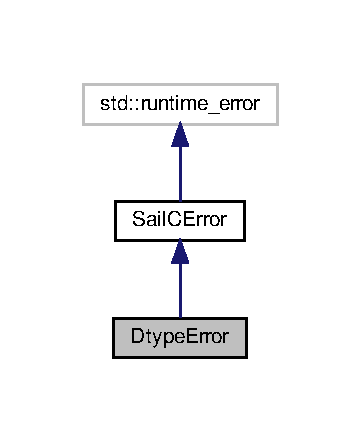
\includegraphics[width=173pt]{classDtypeError__inherit__graph}
\end{center}
\end{figure}


Collaboration diagram for Dtype\+Error\+:\nopagebreak
\begin{figure}[H]
\begin{center}
\leavevmode
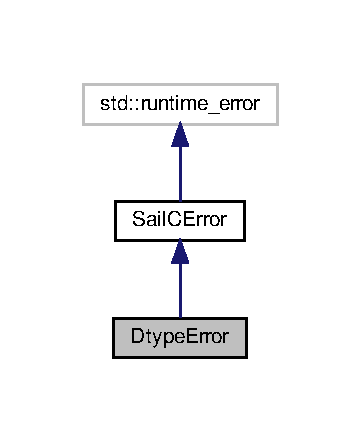
\includegraphics[width=173pt]{classDtypeError__coll__graph}
\end{center}
\end{figure}
\subsection*{Additional Inherited Members}


The documentation for this class was generated from the following file\+:\begin{DoxyCompactItemize}
\item 
/home/tuckersiegel/\+N\+V\+M\+E/sail/sail/csrc/src/error.\+h\end{DoxyCompactItemize}

\hypertarget{structNonPrimitveType}{}\section{Non\+Primitve\+Type$<$ T $>$ Struct Template Reference}
\label{structNonPrimitveType}\index{Non\+Primitve\+Type$<$ T $>$@{Non\+Primitve\+Type$<$ T $>$}}


The documentation for this struct was generated from the following file\+:\begin{DoxyCompactItemize}
\item 
/home/tuckersiegel/\+N\+V\+M\+E/sail/sail/csrc/src/dtypes.\+h\end{DoxyCompactItemize}

\hypertarget{structPrimitiveType}{}\section{Primitive\+Type$<$ T $>$ Struct Template Reference}
\label{structPrimitiveType}\index{Primitive\+Type$<$ T $>$@{Primitive\+Type$<$ T $>$}}


The documentation for this struct was generated from the following file\+:\begin{DoxyCompactItemize}
\item 
/home/tuckersiegel/\+N\+V\+M\+E/sail/sail/csrc/src/dtypes.\+h\end{DoxyCompactItemize}

\hypertarget{classSailCError}{}\section{Sail\+C\+Error Class Reference}
\label{classSailCError}\index{Sail\+C\+Error@{Sail\+C\+Error}}


Inheritance diagram for Sail\+C\+Error\+:\nopagebreak
\begin{figure}[H]
\begin{center}
\leavevmode
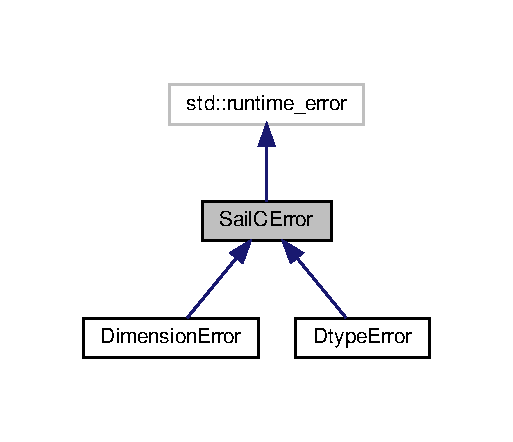
\includegraphics[width=246pt]{classSailCError__inherit__graph}
\end{center}
\end{figure}


Collaboration diagram for Sail\+C\+Error\+:\nopagebreak
\begin{figure}[H]
\begin{center}
\leavevmode
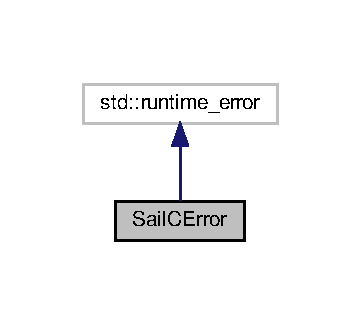
\includegraphics[width=173pt]{classSailCError__coll__graph}
\end{center}
\end{figure}
\subsection*{Public Member Functions}
\begin{DoxyCompactItemize}
\item 
\mbox{\Hypertarget{classSailCError_a25c457ae595ae508ac0e65134a66c6ba}\label{classSailCError_a25c457ae595ae508ac0e65134a66c6ba}} 
{\footnotesize template$<$typename... Args$>$ }\\{\bfseries Sail\+C\+Error} (const Args \&... args)
\end{DoxyCompactItemize}


The documentation for this class was generated from the following file\+:\begin{DoxyCompactItemize}
\item 
/home/tuckersiegel/\+N\+V\+M\+E/sail/sail/csrc/src/error.\+h\end{DoxyCompactItemize}

\hypertarget{classsail_1_1Tensor}{}\section{sail\+:\+:Tensor Class Reference}
\label{classsail_1_1Tensor}\index{sail\+::\+Tensor@{sail\+::\+Tensor}}


Collaboration diagram for sail\+:\+:Tensor\+:\nopagebreak
\begin{figure}[H]
\begin{center}
\leavevmode
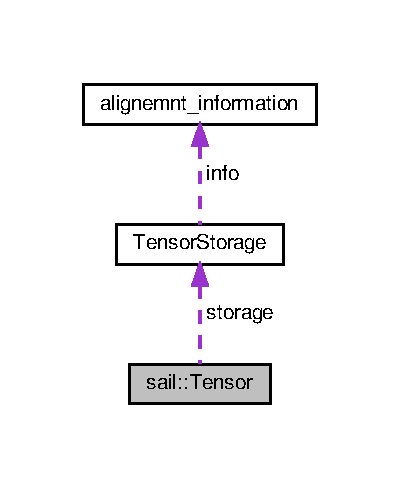
\includegraphics[width=192pt]{classsail_1_1Tensor__coll__graph}
\end{center}
\end{figure}
\subsection*{Public Member Functions}
\begin{DoxyCompactItemize}
\item 
\mbox{\Hypertarget{classsail_1_1Tensor_a777bfdb1dd5215532066436924e03856}\label{classsail_1_1Tensor_a777bfdb1dd5215532066436924e03856}} 
{\bfseries Tensor} (\hyperlink{classTensorStorage}{Tensor\+Storage} storage)
\item 
\mbox{\Hypertarget{classsail_1_1Tensor_a127524df8b657c0109086a3a78779c34}\label{classsail_1_1Tensor_a127524df8b657c0109086a3a78779c34}} 
{\bfseries Tensor} (int \&ndims, void $\ast$\&data, Dtype \&dt, Tensor\+Size \&strides, Tensor\+Size \&shape)
\item 
\mbox{\Hypertarget{classsail_1_1Tensor_ab502ae2dc23e1aa444f572dab0114c8b}\label{classsail_1_1Tensor_ab502ae2dc23e1aa444f572dab0114c8b}} 
void {\bfseries reshape} (const Tensor\+Size s)
\item 
\mbox{\Hypertarget{classsail_1_1Tensor_af8f4518676aae8f6a1769f42e125afaf}\label{classsail_1_1Tensor_af8f4518676aae8f6a1769f42e125afaf}} 
\hyperlink{classsail_1_1Tensor}{Tensor} {\bfseries expand\+\_\+dims} (const int dim)
\item 
\mbox{\Hypertarget{classsail_1_1Tensor_a98fd1ee5178b969cdd4b45a284759325}\label{classsail_1_1Tensor_a98fd1ee5178b969cdd4b45a284759325}} 
void $\ast$ {\bfseries data} ()
\item 
\mbox{\Hypertarget{classsail_1_1Tensor_a50a27e137b38b4a0fa7733df8c23f4ab}\label{classsail_1_1Tensor_a50a27e137b38b4a0fa7733df8c23f4ab}} 
bool {\bfseries is\+Scalar} ()
\item 
\mbox{\Hypertarget{classsail_1_1Tensor_a6cf97b740b9a866db2be07aa5da4c810}\label{classsail_1_1Tensor_a6cf97b740b9a866db2be07aa5da4c810}} 
Dtype {\bfseries dtype} ()
\item 
\mbox{\Hypertarget{classsail_1_1Tensor_a87b1a7e15afb7b621bc99828c78ad4b7}\label{classsail_1_1Tensor_a87b1a7e15afb7b621bc99828c78ad4b7}} 
void {\bfseries free} ()
\item 
\mbox{\Hypertarget{classsail_1_1Tensor_a770d2fd4f131da42a50d5790af21255a}\label{classsail_1_1Tensor_a770d2fd4f131da42a50d5790af21255a}} 
long int $\ast$ {\bfseries get\+Shape\+Ptr} ()
\item 
\mbox{\Hypertarget{classsail_1_1Tensor_a70b06adbeb2b2b9567fbf9fa615ebd1b}\label{classsail_1_1Tensor_a70b06adbeb2b2b9567fbf9fa615ebd1b}} 
int {\bfseries get\+N\+P\+Type\+Num} ()
\item 
\mbox{\Hypertarget{classsail_1_1Tensor_af3f9e9beaa195d6a48cd523d531d8ce4}\label{classsail_1_1Tensor_af3f9e9beaa195d6a48cd523d531d8ce4}} 
\hyperlink{classsail_1_1Tensor}{Tensor} {\bfseries operator+} (const \hyperlink{classsail_1_1Tensor}{Tensor} \&t)
\item 
\mbox{\Hypertarget{classsail_1_1Tensor_af832582e453597ae2d363d0936abc77a}\label{classsail_1_1Tensor_af832582e453597ae2d363d0936abc77a}} 
\hyperlink{classsail_1_1Tensor}{Tensor} {\bfseries operator-\/} (const \hyperlink{classsail_1_1Tensor}{Tensor} \&t)
\item 
\mbox{\Hypertarget{classsail_1_1Tensor_afaa6db9a39f505b4f796349fcc17a19e}\label{classsail_1_1Tensor_afaa6db9a39f505b4f796349fcc17a19e}} 
\hyperlink{classsail_1_1Tensor}{Tensor} {\bfseries operator$\ast$} (const \hyperlink{classsail_1_1Tensor}{Tensor} \&t)
\item 
\mbox{\Hypertarget{classsail_1_1Tensor_a937b0da33dfb53b1c111a773c0b9ef88}\label{classsail_1_1Tensor_a937b0da33dfb53b1c111a773c0b9ef88}} 
\hyperlink{classsail_1_1Tensor}{Tensor} {\bfseries operator/} (const \hyperlink{classsail_1_1Tensor}{Tensor} \&t)
\item 
\mbox{\Hypertarget{classsail_1_1Tensor_ae9bbb41d1a9f6c1c0a2241301059effd}\label{classsail_1_1Tensor_ae9bbb41d1a9f6c1c0a2241301059effd}} 
\hyperlink{classsail_1_1Tensor}{Tensor} {\bfseries operator\mbox{[}$\,$\mbox{]}} (const int t)
\item 
\mbox{\Hypertarget{classsail_1_1Tensor_a237adf4c39950d5a56b3a7b608cadfb6}\label{classsail_1_1Tensor_a237adf4c39950d5a56b3a7b608cadfb6}} 
\hyperlink{classsail_1_1Tensor}{Tensor} {\bfseries sum} ()
\end{DoxyCompactItemize}
\subsection*{Static Public Member Functions}
\begin{DoxyCompactItemize}
\item 
\mbox{\Hypertarget{classsail_1_1Tensor_a9a798c58a36c12db832739235f330b9d}\label{classsail_1_1Tensor_a9a798c58a36c12db832739235f330b9d}} 
static \hyperlink{classsail_1_1Tensor}{Tensor} {\bfseries create\+Empty\+Scalar} (Dtype dt)
\end{DoxyCompactItemize}
\subsection*{Public Attributes}
\begin{DoxyCompactItemize}
\item 
\mbox{\Hypertarget{classsail_1_1Tensor_a998b6320f8aa40363d242b2bcd83be7b}\label{classsail_1_1Tensor_a998b6320f8aa40363d242b2bcd83be7b}} 
\hyperlink{classTensorStorage}{Tensor\+Storage} {\bfseries storage}
\end{DoxyCompactItemize}


The documentation for this class was generated from the following files\+:\begin{DoxyCompactItemize}
\item 
/home/tuckersiegel/\+N\+V\+M\+E/sail/sail/csrc/src/Tensor.\+h\item 
/home/tuckersiegel/\+N\+V\+M\+E/sail/sail/csrc/src/Tensor.\+cpp\end{DoxyCompactItemize}

\hypertarget{classTensorStorage}{}\section{Tensor\+Storage Class Reference}
\label{classTensorStorage}\index{Tensor\+Storage@{Tensor\+Storage}}


Collaboration diagram for Tensor\+Storage\+:\nopagebreak
\begin{figure}[H]
\begin{center}
\leavevmode
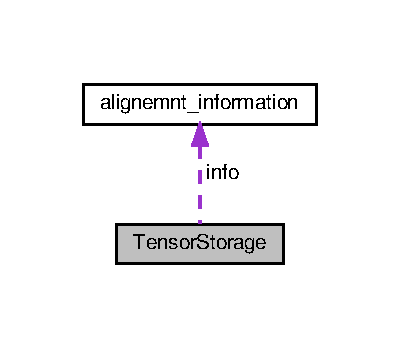
\includegraphics[width=192pt]{classTensorStorage__coll__graph}
\end{center}
\end{figure}
\subsection*{Public Member Functions}
\begin{DoxyCompactItemize}
\item 
\mbox{\Hypertarget{classTensorStorage_a185e38a60bf24d574dfa2030275bbd02}\label{classTensorStorage_a185e38a60bf24d574dfa2030275bbd02}} 
{\bfseries Tensor\+Storage} (int nd, void $\ast$in\+\_\+data, int64\+\_\+t in\+\_\+offset, Dtype dt, Tensor\+Shape st, Tensor\+Shape sh)
\item 
\mbox{\Hypertarget{classTensorStorage_a687c22d0f1c4ca429feb2b354096429e}\label{classTensorStorage_a687c22d0f1c4ca429feb2b354096429e}} 
void {\bfseries reshape} (const Tensor\+Size new\+\_\+shape)
\item 
\mbox{\Hypertarget{classTensorStorage_ac2016f8cbd28d2382a505177afe78323}\label{classTensorStorage_ac2016f8cbd28d2382a505177afe78323}} 
void {\bfseries expand\+\_\+dims} (const int dim)
\item 
\mbox{\Hypertarget{classTensorStorage_a8667175f454eb36f70dc7e9dfc185ad4}\label{classTensorStorage_a8667175f454eb36f70dc7e9dfc185ad4}} 
void {\bfseries free\+\_\+data} ()
\item 
\mbox{\Hypertarget{classTensorStorage_afe0e9c666e89dea2fe69c97ffcd4a4c9}\label{classTensorStorage_afe0e9c666e89dea2fe69c97ffcd4a4c9}} 
void $\ast$ {\bfseries operator\mbox{[}$\,$\mbox{]}} (int index)
\item 
\mbox{\Hypertarget{classTensorStorage_a3a4116b14541e8cae21110db98f5f7f5}\label{classTensorStorage_a3a4116b14541e8cae21110db98f5f7f5}} 
Tensor\+Size {\bfseries get\+Shape} ()
\item 
\mbox{\Hypertarget{classTensorStorage_a239fb3bb35fb9db89b8413041c038654}\label{classTensorStorage_a239fb3bb35fb9db89b8413041c038654}} 
std\+::string {\bfseries get\+Shape\+String} ()
\item 
\mbox{\Hypertarget{classTensorStorage_ab32ca2aaa137c68c0c3ceea76575022f}\label{classTensorStorage_ab32ca2aaa137c68c0c3ceea76575022f}} 
std\+::string {\bfseries get\+Stridetring} ()
\item 
\mbox{\Hypertarget{classTensorStorage_acb84883442f719b2d7aeda4dd743ef20}\label{classTensorStorage_acb84883442f719b2d7aeda4dd743ef20}} 
std\+::vector$<$ Tensor\+Size $>$ {\bfseries step\+\_\+back} ()
\item 
\mbox{\Hypertarget{classTensorStorage_a934218af682e938ebe22e89b2ae5edf4}\label{classTensorStorage_a934218af682e938ebe22e89b2ae5edf4}} 
size\+\_\+t {\bfseries get\+Dtype\+Size} ()
\item 
\mbox{\Hypertarget{classTensorStorage_a618069b19b2b9171d6b07d874696cf27}\label{classTensorStorage_a618069b19b2b9171d6b07d874696cf27}} 
size\+\_\+t {\bfseries get\+Total\+Size} ()
\item 
\mbox{\Hypertarget{classTensorStorage_a21a43d53a12ce9a37e02909ead533c8f}\label{classTensorStorage_a21a43d53a12ce9a37e02909ead533c8f}} 
int {\bfseries numel} () const
\end{DoxyCompactItemize}
\subsection*{Static Public Member Functions}
\begin{DoxyCompactItemize}
\item 
\mbox{\Hypertarget{classTensorStorage_adc86cd3668de177f7f53895405d602f5}\label{classTensorStorage_adc86cd3668de177f7f53895405d602f5}} 
static \hyperlink{classTensorStorage}{Tensor\+Storage} {\bfseries create\+Empty} (int nd, void $\ast$in\+\_\+data, int64\+\_\+t in\+\_\+offset, Dtype dt, Tensor\+Size st, Tensor\+Size sh)
\item 
\mbox{\Hypertarget{classTensorStorage_a7efa8bff4fad4642f035a28de2e0b494}\label{classTensorStorage_a7efa8bff4fad4642f035a28de2e0b494}} 
static \hyperlink{classTensorStorage}{Tensor\+Storage} {\bfseries create\+Empty} (int nd, void $\ast$in\+\_\+data, int64\+\_\+t in\+\_\+offset, Dtype dt, Tensor\+Size st, Tensor\+Size sh, \hyperlink{structalignemnt__information}{alignemnt\+\_\+information} i)
\item 
\mbox{\Hypertarget{classTensorStorage_a91968d3da292d7069839e13ab9307110}\label{classTensorStorage_a91968d3da292d7069839e13ab9307110}} 
static void {\bfseries check\+\_\+dimensions\+\_\+elementwise} (\hyperlink{classTensorStorage}{Tensor\+Storage} a, \hyperlink{classTensorStorage}{Tensor\+Storage} b)
\end{DoxyCompactItemize}
\subsection*{Public Attributes}
\begin{DoxyCompactItemize}
\item 
\mbox{\Hypertarget{classTensorStorage_a1288f01bbdaa9f55e685acc2df76b364}\label{classTensorStorage_a1288f01bbdaa9f55e685acc2df76b364}} 
int {\bfseries arr\+\_\+numel}
\item 
\mbox{\Hypertarget{classTensorStorage_ac18d1ac2fe325bc1ae3bc988cb9058c2}\label{classTensorStorage_ac18d1ac2fe325bc1ae3bc988cb9058c2}} 
int {\bfseries ndim}
\item 
\mbox{\Hypertarget{classTensorStorage_a20ff45e34fbaa71b705f48b0706d1898}\label{classTensorStorage_a20ff45e34fbaa71b705f48b0706d1898}} 
Dtype {\bfseries dtype}
\item 
\mbox{\Hypertarget{classTensorStorage_a175bc84e9fef71edb10e9e8a7473ac82}\label{classTensorStorage_a175bc84e9fef71edb10e9e8a7473ac82}} 
void $\ast$ {\bfseries data}
\item 
\mbox{\Hypertarget{classTensorStorage_a82acc1fa796de34ac62930be0e3e1c99}\label{classTensorStorage_a82acc1fa796de34ac62930be0e3e1c99}} 
int64\+\_\+t {\bfseries offset}
\item 
\mbox{\Hypertarget{classTensorStorage_a9d62e01a2163a8c4d4efbfc2b9e1076f}\label{classTensorStorage_a9d62e01a2163a8c4d4efbfc2b9e1076f}} 
Tensor\+Size {\bfseries strides}
\item 
\mbox{\Hypertarget{classTensorStorage_a547b231dcfbc9c679860661a4e2291f6}\label{classTensorStorage_a547b231dcfbc9c679860661a4e2291f6}} 
Tensor\+Size {\bfseries shape}
\item 
\mbox{\Hypertarget{classTensorStorage_a6d31da541697683ab7505bf42542d544}\label{classTensorStorage_a6d31da541697683ab7505bf42542d544}} 
\hyperlink{structalignemnt__information}{alignemnt\+\_\+information} {\bfseries info}
\end{DoxyCompactItemize}


The documentation for this class was generated from the following file\+:\begin{DoxyCompactItemize}
\item 
/home/tuckersiegel/\+N\+V\+M\+E/sail/sail/csrc/src/Tensor\+\_\+storage.\+h\end{DoxyCompactItemize}

%--- End generated contents ---

% Index
\backmatter
\newpage
\phantomsection
\clearemptydoublepage
\addcontentsline{toc}{chapter}{Index}
\printindex

\end{document}
